\documentclass{beamer}

% Theme
\usetheme{Madrid}
\usecolortheme{default}

% Packages
\usepackage{amsmath,amssymb,amsfonts}
\usepackage{graphicx}
\usepackage{xcolor}
\usepackage{tikz}
\usepackage{tkz-euclide}
\usepackage{array}
\usepackage{multirow}
\usepackage{longtable}
\usepackage{lscape}
\usepackage{listings}
\lstset{
    basicstyle=\ttfamily\small,
    keywordstyle=\color{blue},
    commentstyle=\color{gray},
    stringstyle=\color{red},
    showstringspaces=false,
    breaklines=true
}



% Custom macros
\newcommand{\myvec}[1]{\begin{pmatrix}#1\end{pmatrix}}
\newcommand{\brak}[1]{\left( #1 \right)}

% Redefine \vec to bold letters only (no arrow)
\renewcommand{\vec}[1]{\mathbf{#1}}

\title{4.13.24}
\author{EE25BTECH11019 -- Darji Vivek M.}
\date{}

\begin{document}

\begin{frame}
\begin{titlepage}

\end{titlepage}
\end{frame}

\begin{frame}{Question}
\textbf{Question:}\\
The number of points, having both coordinates as integers, that lie in the interior of the triangle with vertices 
\[
(0,0), \quad (0,41), \quad (41,0)
\]
is?
\begin{enumerate}
    \item 820
    \item 780
    \item 901
    \item 861
\end{enumerate}
\end{frame}

\begin{frame}{Solution:Represent vertices and Area using determinant}
\begin{align}
\vec{A} &= \myvec{0\\0}, &
\vec{B} &= \myvec{0\\41}, &
\vec{C} &= \myvec{41\\0}
\end{align}

\begin{align}
A &= \frac{1}{2}\left|\begin{vmatrix}0 & 41\\41 & 0\end{vmatrix}\right|\\
A &= \frac{1}{2}\left|0 - (41)(41)\right|\\
A &= \frac{1681}{2}
\end{align}
\end{frame}

\begin{frame}{Solution:Boundary lattice points formula}
For a line joining integer points \((x_1,y_1)\) and \((x_2,y_2)\),  
the number of lattice points on it is
\[
N = \gcd(|x_2-x_1|, |y_2-y_1|) + 1
\]

\textbf{Compute for each side:}
\begin{align}
B_1 &= \gcd(|0-0|, |41-0|) + 1 = 42 \\ 
B_2 &= \gcd(|41-0|, |0-0|) + 1 = 42 \\ 
B_3 &= \gcd(|41-0|, |0-41|) + 1 = 42
\end{align}
Each vertex is counted twice, so
\[
B = 42 + 42 + 42 - 3 = 123
\]
\end{frame}

\begin{frame}{Solution:Apply Pick's Theorem}
Pick's theorem:
\[
A = I + \frac{B}{2} - 1
\]
Rearranging for interior points \(I\):
\[
I = A - \frac{B}{2} + 1
\]
\end{frame}

\begin{frame}{Solution:Substitute values and Answer}
\begin{align}
I &= \frac{1681}{2} - \frac{123}{2} + 1\\
I &= \frac{1558}{2} + 1\\
I &= 780
\end{align}
The number of integer lattice points lying strictly inside the triangle is
\[
\boxed{780}
\]
\end{frame}

\begin{frame}[fragile]{C Code}
\begin{lstlisting}
#include <stdio.h>
#include <stdlib.h>

// Function to find GCD (used for boundary lattice points)
int gcd(int a, int b) {
    if (b == 0)
        return a;
    return gcd(b, a % b);
}

// Function to find number of boundary points on one edge
int boundary_points(int x1, int y1, int x2, int y2) {
    return gcd(abs(x2 - x1), abs(y2 - y1)) + 1;
}

// Function to find total interior lattice points using Pick's theorem
\end{lstlisting}
\end{frame}

\begin{frame}[fragile]{C Code}
\begin{lstlisting}
int interior_points(int x1, int y1, int x2, int y2, int x3, int y3) {
    // Area = 1/2 * |x1(y2 - y3) + x2(y3 - y1) + x3(y1 - y2)|
    float area = 0.5 * (float)abs(x1*(y2 - y3) + x2*(y3 - y1) + x3*(y1 - y2));
    // Boundary points on all three sides
    int b1 = boundary_points(x1, y1, x2, y2);
    int b2 = boundary_points(x2, y2, x3, y3);
    int b3 = boundary_points(x3, y3, x1, y1);
    // Subtract 3 since each vertex is counted twice
    int B = b1 + b2 + b3 - 3;
    // Pick's theorem: A = I + B/2 - 1  =>  I = A - B/2 + 1
    int I = (int)(area - (float)B/2 + 1);

    return I;
}
\end{lstlisting}
\end{frame}

\begin{frame}[fragile]{Python (Call)}
\begin{lstlisting}[language=Python]
import ctypes
import numpy as np
import matplotlib.pyplot as plt
# Load the compiled C library
lib = ctypes.CDLL('./9.so')
# Define argument and return types
lib.interior_points.argtypes = [ctypes.c_int, ctypes.c_int, ctypes.c_int, ctypes.c_int, ctypes.c_int, ctypes.c_int]
lib.interior_points.restype = ctypes.c_int
# Triangle vertices
x1, y1 = 0, 0
x2, y2 = 0, 41
x3, y3 = 41, 0
# Call C function to get interior lattice points
I = lib.interior_points(x1, y1, x2, y2, x3, y3)
print("Number of interior lattice points:", I)
\end{lstlisting}
\end{frame}

\begin{frame}[fragile]{Python (Call)}
\begin{lstlisting}[language=Python]
# ---- Generate interior points ----
points = []
for i in range(42):
    for j in range(42):
        if i > 0 and j > 0 and i + j < 41:
            points.append((i, j))
pts = np.array(points)
x, y = pts[:, 0], pts[:, 1]

# ---- Plotting ----
plt.figure(figsize=(6,6))
plt.plot([x1, x2, x3, x1], [y1, y2, y3, y1], 'k-', label="Triangle")
plt.scatter(x, y, s=10, color='red', label="Interior Lattice Points")
\end{lstlisting}
\end{frame}

\begin{frame}[fragile]{Python (Call)}
\begin{lstlisting}[language=Python]
# Label the vertices with coordinates
plt.text(x1, y1, f"({x1},{y1})", fontsize=10, verticalalignment='bottom', horizontalalignment='right')
plt.text(x2, y2, f"({x2},{y2})", fontsize=10, verticalalignment='bottom', horizontalalignment='left')
plt.text(x3, y3, f"({x3},{y3})", fontsize=10, verticalalignment='top', horizontalalignment='right')

plt.title("Integer Lattice Points Inside Triangle")
plt.xlabel("x")
plt.ylabel("y")
plt.legend()
plt.axis('equal')
plt.grid(True)
plt.show()
\end{lstlisting}
\end{frame}
\begin{frame}{Python Output and Plot}
\begin{figure}[h!]
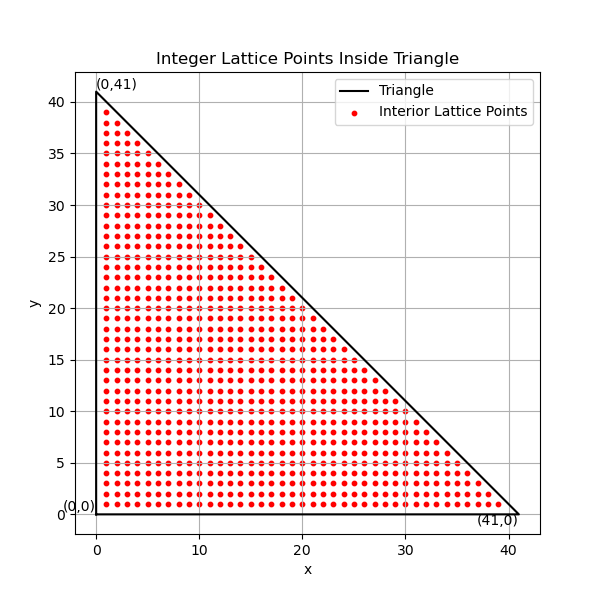
\includegraphics[width=0.70\columnwidth]{figs/9.png}
\caption{}
\end{figure}
\end{frame}
\end{document}